% Appendix A

\chapter{OFDR traces}
\label{ch:appendixA}
 \autoref{fig:couplerA}, \autoref{fig:couplerB} and \autoref{fig:couplerC} represent the ODFR traces acquired for determining the length of the arms of the three fiber couplers, as discussed in \autoref{ch:setup}. The title on top of each graph indicates the corresponding input port, while the color of the traces refers to the port which was connected to the patch cord (black is used  instead of white).
 
\begin{figure}[hbt]
	\myfloatalign
	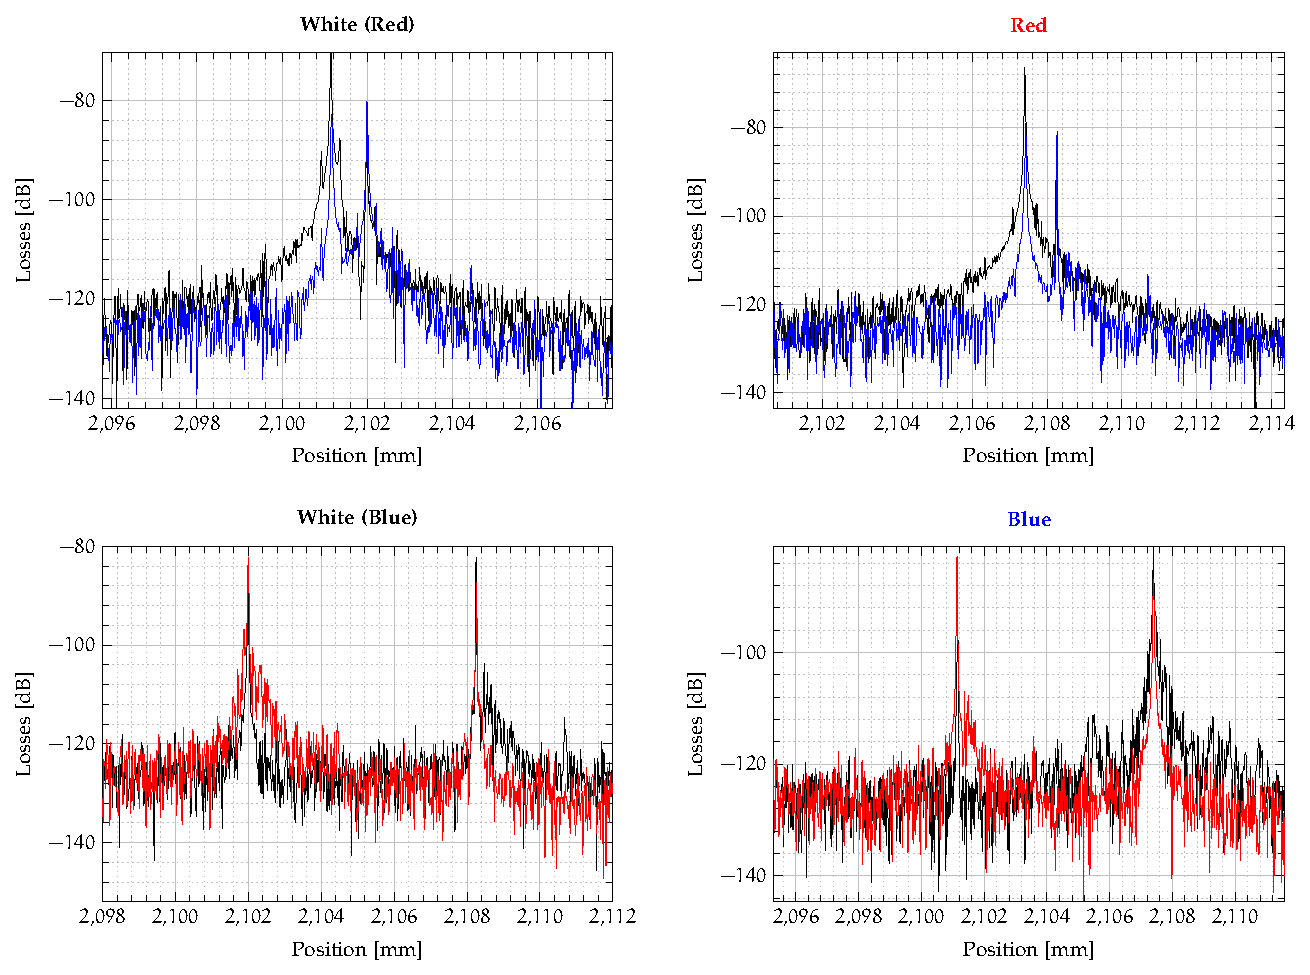
\includegraphics[width=\linewidth]{gfx/ch3/couplers/couplerA}
	\caption{OFDR traces of the first 50-50 coupler (Coupler A).}\label{fig:couplerA}
\end{figure}

\begin{figure}[hbt]
	\myfloatalign
	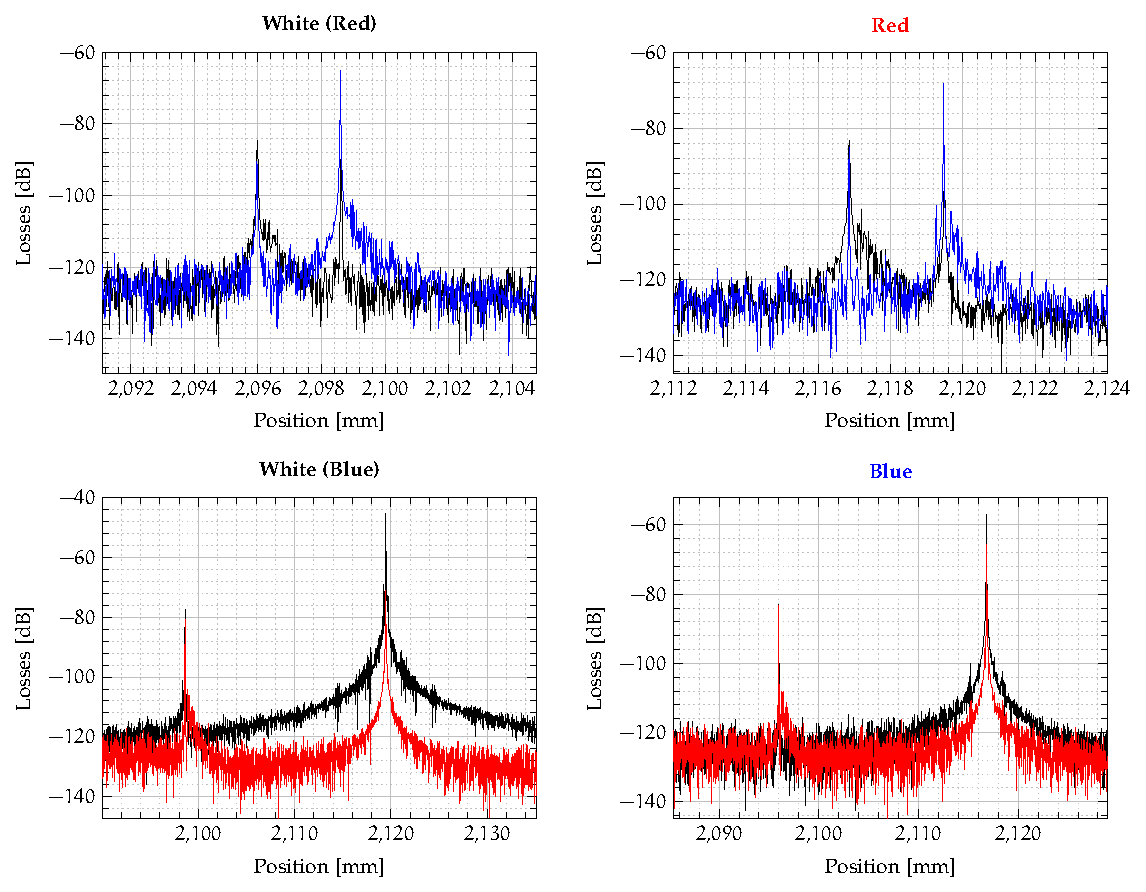
\includegraphics[width=\linewidth]{gfx/ch3/couplers/couplerB}
	\caption{OFDR traces of the second 50-50 coupler (Coupler B).}\label{fig:couplerB}
\end{figure}

\begin{figure}[hbt]
	\myfloatalign
	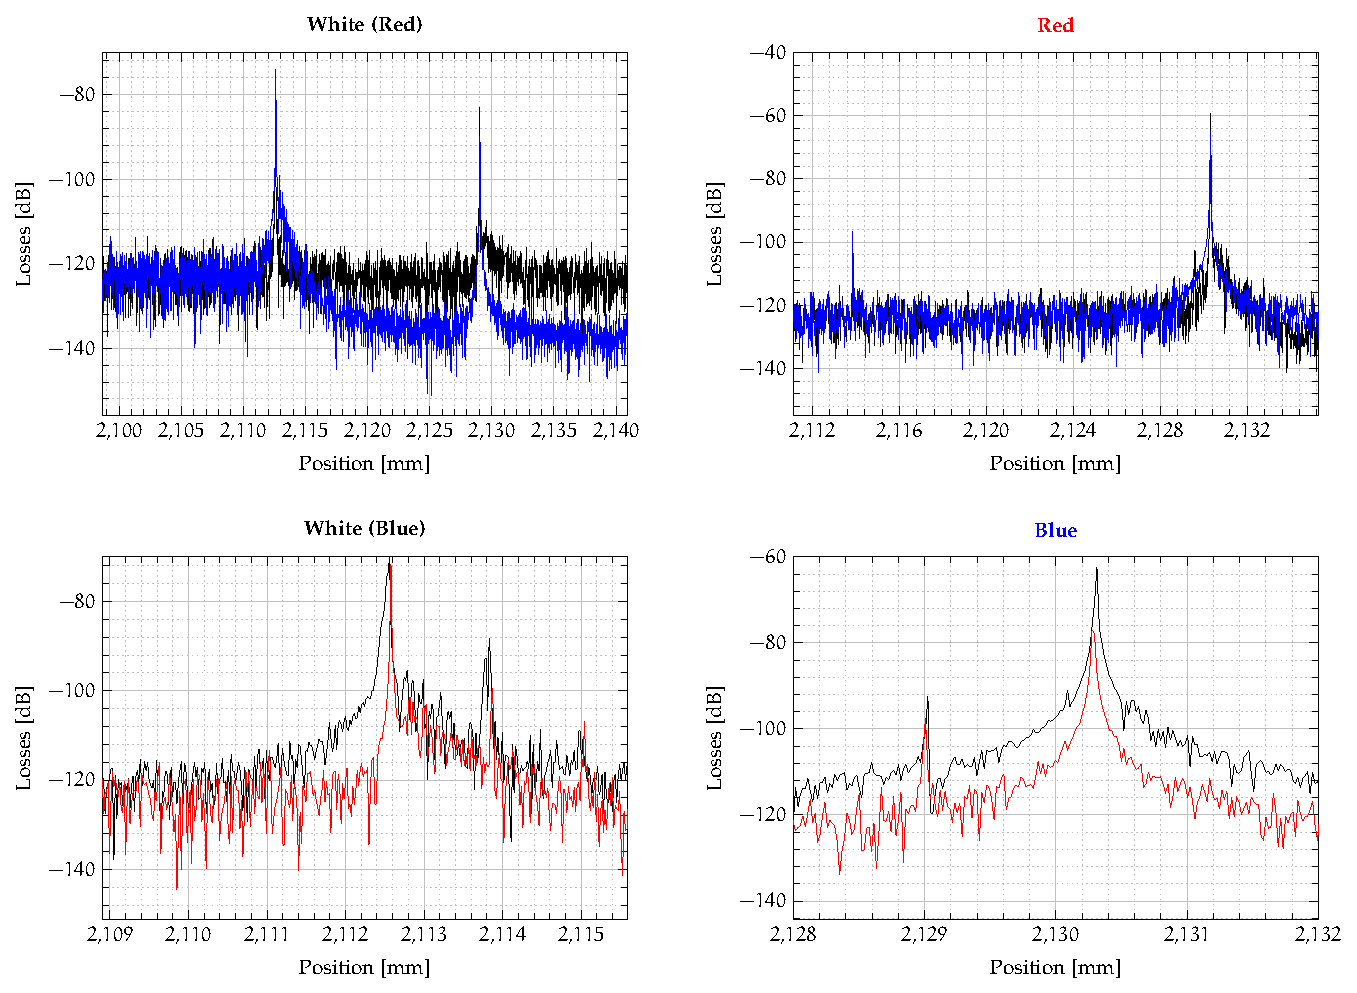
\includegraphics[width=\linewidth]{gfx/ch3/couplers/couplerC}
	\caption{OFDR traces of the 90-10 coupler.}\label{fig:couplerC}
\end{figure}


\section{Appendix Section Test}
\graffito{More dummy text}

%----------------------------------------------------------------------------------------
\section{Another Appendix Section Test}

\begin{table}
\myfloatalign
\begin{tabularx}{\textwidth}{Xll} \toprule
\tableheadline{labitur bonorum pri no} & \tableheadline{que vista}
& \tableheadline{human} \\ \midrule
fastidii ea ius & germano &  demonstratea \\
suscipit instructior & titulo & personas \\
\midrule
quaestio philosophia & facto & demonstrated \\
\bottomrule
\end{tabularx}
\caption[Autem usu id]{Autem usu id.}
\label{tab:moreexample}
\end{table}


There is also a useless Pascal listing below: \autoref{lst:useless}.

\begin{lstlisting}[float=b,language=C,frame=tb,caption={A floating example (\texttt{listings} manual)},label=lst:useless]

int index = 0;
float timeout = 2000;
while (! stopAcquisition)
{
	index = index mod buffercount
	
	short integer* buffer = AlazarWaitBuffer(bufferArray[index], timeout);
	
	float* toDisk = processBuffer(buffer);
	byte*  Bscan = createBitmap(buffer);
	
	emit newBuffer(toDisk);
	emit newFrame(Bscan);
	
	index++;
}
\end{lstlisting}
